\section{Introduction}\label{sec:1}

\subsection{Background}\label{sec:1.1}

The basic oxygen converter turns hot metal into steel by blowing high-purity oxygen through a lance at supersonic speed. Silicon, manganese, phosphorus and carbon are oxidized in turn, and the carbon leaves the bath as CO and CO\ensuremath{_{2}}. Operators must time the end of the blow so that the carbon content and temperature of the steel reach their targets together \cite{ref:11}. They therefore follow the progress of decarburization from two sources. A spectrometer at the converter mouth records the flame radiation every 0.5 s, and a Raman analyzer at the flue-gas bend records the CO and CO\ensuremath{_{2}} contents at the same rate.

The two sources see the same reactions at different times. The flame responds to the bath immediately, while the gas must travel through the hood and the duct before the analyzer can measure it. This transport delay limits endpoint control, because a decision based on the analyzer refers to a bath state that is already half a minute old. The sampling probe also wears quickly in the dusty, high-temperature duct, so frequent sampling is costly. A data-driven soft sensor that reads the off-gas state from the flame \cite{ref:12,ref:13} would provide the signal earlier and would allow the probe to work less often.

Figure~\ref{fig:1} shows the two measurement locations.
\begin{figure}[!htbp]
\centering
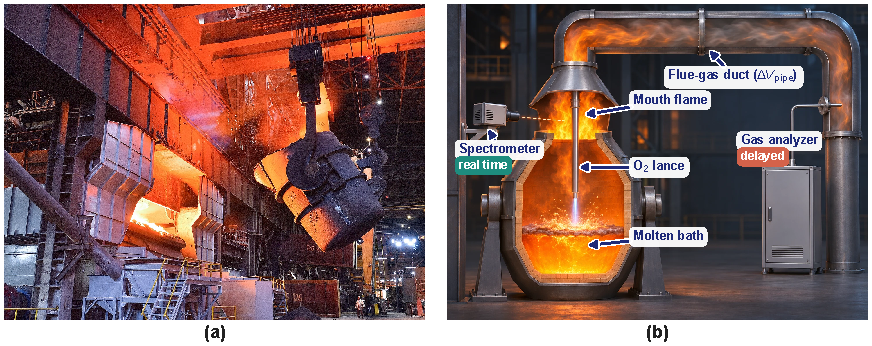
\includegraphics[width=0.7\linewidth]{figures/fig01_dual_modal_schematic.pdf}
\caption{Dual-modal sensing layout of the basic oxygen converter.}\label{fig:1}
\end{figure}

\subsection{Restatement of the Problem}\label{sec:1.2}

The problem provides the full-process flame spectra (2,047 wavelengths, 0.5-s step), the cumulative oxygen consumption and the CO and CO\ensuremath{_{2}} signals of ten heats. We address the following tasks.

\begin{itemize}
\item \textbf{Task 1.} Remove the outliers in the spectral data, reconstruct a continuous spectral surface, and draw the three-dimensional spectra of all ten heats.
\item \textbf{Task 2.} Remove the outliers in the oxygen and gas series, reconstruct continuous curves of the lance flow, cumulative oxygen, CO, CO\ensuremath{_{2}} and their cumulative emissions, relate the gas signals to the oxygen consumption, and compute the flue-gas delay under different lance flow rates.
\item \textbf{Task 3.} Use the results of Tasks 1 and 2 to predict the flue-gas information in real time from the flame spectra, and test the prediction on all ten heats.
\item \textbf{Combination requirement.} Combine the models learned from different heats, as a whole or by groups, so that the combined model performs well on all ten heats.
\end{itemize}

\subsection{Our Work}\label{sec:1.3}

Figure~\ref{fig:2} outlines our workflow. We first diagnose the data and resolve four inconsistencies that would otherwise distort every downstream step. Section~\ref{sec:4} then introduces an arrival-time map linking each real-time flame observation to the delayed gas reading it generates. The three tasks proceed as an integrated pipeline. First, Task 1 builds a low-rank model of the flame spectra to remove outliers and supply cleaned spectral representations. Second, Task 2 reconstructs the process curves, partitions each blow into chemical stages and quantifies how transport delay varies with lance flow. Finally, Task 3 feeds a spectral basis built on the low-rank structure of Task 1 and the delay map from Task 2 into a causal real-time predictor. It combines the heat-level models and updates predictions whenever a probe reading arrives.

\begin{figure}[!htbp]
\centering
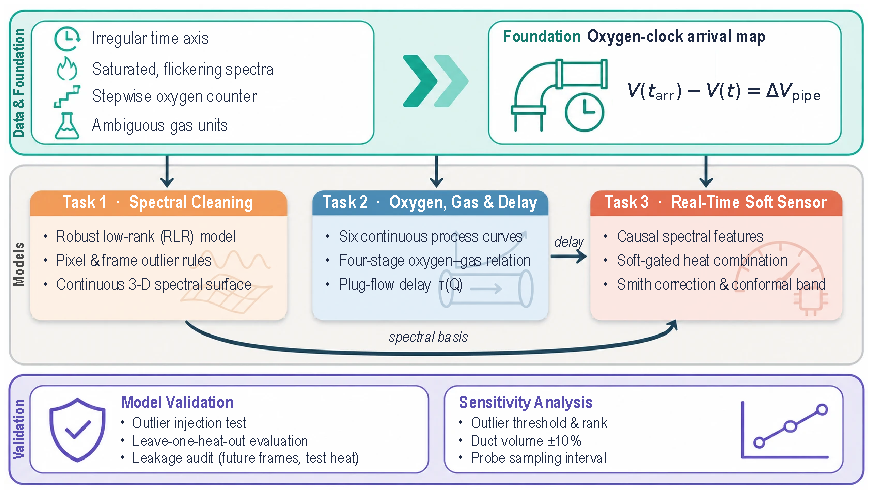
\includegraphics[width=1.0\linewidth]{figures/fig02_framework.pdf}
\caption{Integrated modeling framework across Tasks 1–3.}\label{fig:2}
\end{figure}


\FloatBarrier
\section{Assumptions and Notation}\label{sec:2}

\subsection{Assumptions}\label{sec:2.1}

\textbf{Assumption 1. The gas in the duct moves as a plug flow with mild mixing.} \emph{Justification:} the duct is long and narrow compared with its diameter, so axial mixing is small relative to transport \cite{ref:10}. We represent the remaining mixing by a first-order lag and test its time constant in Section~\ref{sec:8}.

\textbf{Assumption 2. The flue-gas flow is proportional to the lance oxygen flow.} \emph{Justification:} decarburization consumes most of the blown oxygen during the main blow, so the gas generated per second scales with the oxygen supplied per second. This assumption lets Section~\ref{sec:4} measure the duct in oxygen units.

\textbf{Assumption 3. The spectrometer has no measurement delay.} \emph{Justification:} the flame is observed optically at the converter mouth, and the optical response is far faster than the 0.5-s sampling step. The flame therefore serves as the real-time reference in Sections 6 and 7.

\textbf{Assumption 4. The analyzer reports volume fractions.} \emph{Justification:} Section~\ref{sec:3.4} shows that the flow-rate reading violates the carbon–oxygen balance by a factor of about six, whereas the volume-fraction reading agrees with the typical composition of converter gas.

\textbf{Assumption 5. Frame-to-frame flame flicker is random variation around a trend.} \emph{Justification:} turbulent combustion at the converter mouth drives rapid flicker that neighbouring frames cannot predict (Section~\ref{sec:5.2.2}). We therefore treat flicker as a residual rather than as a signal to reproduce.

\subsection{Notation}\label{sec:2.2}

Table~\ref{tab:1} lists the symbols and their units.
\begin{table}[!htbp]
\centering\small
\caption{Notation}\label{tab:1}
\renewcommand{\arraystretch}{1.12}
\begin{tabularx}{\linewidth}{@{}c Z c@{}}
\toprule
\textbf{Symbol} & \textbf{Description} & \textbf{Unit} \\
\midrule
$k$ & heat index, $k = 1,\dots,10$ & – \\
$I(t,\lambda)$ & flame intensity at time $t$ and wavelength $\lambda$ & counts \\
$\mathbf{X}$ & log-intensity matrix (time \ensuremath{\times} wavelength) & – \\
$\mathbf{L},\ \mathbf{S}$ & low-rank and sparse parts of $\mathbf{X}$ & – \\
$r$ & rank of $\mathbf{L}$ & – \\
$V(t)$ & cumulative oxygen consumption & m\ensuremath{^{3}} \\
$Q(t)$ & lance oxygen flow, $Q = \mathrm{d}V/\mathrm{d}t$ & m\ensuremath{^{3}}/s \\
$y_{\mathrm{CO}}(t),\ y_{\mathrm{CO_2}}(t)$ & CO and CO\ensuremath{_{2}} readings of the analyzer & vol.\% \\
$E_{\mathrm{CO}}(t),\ E_{\mathrm{CO_2}}(t)$ & time integrals of the readings & as in data \\
$\Delta V_{\mathrm{pipe}}$ & equivalent duct volume, in oxygen units & m\ensuremath{^{3}} \\
$T_{\mathrm{mix}}$ & mixing time constant & s \\
$\tau(Q)$ & flue-gas delay at lance flow $Q$ & s \\
$t_{\mathrm{arr}}(t)$ & time at which gas generated at $t$ reaches the analyzer & s \\
$\hat{y}(t)$ & real-time prediction of the delay-aligned reading & vol.\% \\
$N_{\mathrm{p}}$ & probe sampling interval & s \\
\bottomrule
\end{tabularx}
\end{table}


\FloatBarrier
\section[Data Preprocessing and Consistency]{Data Preprocessing and Consistency Diagnosis}\label{sec:3}

Each attachment contains about 1,400 spectra of 2,047 wavelengths and the corresponding oxygen and gas records. Every model in this paper depends on the time axis, the lance flow and the meaning of the gas readings, so we examine these three items before modelling. Figure~\ref{fig:3} shows the workflow, and Table~\ref{tab:2} summarizes the ten heats after preprocessing.

\begin{figure}[!htbp]
\centering
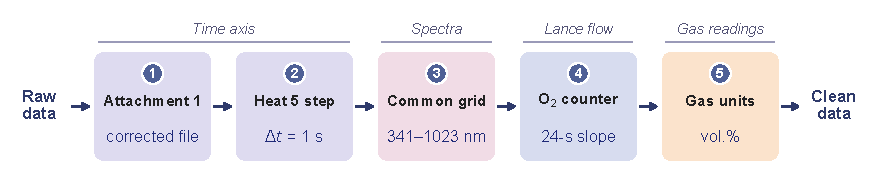
\includegraphics[width=1.0\linewidth]{figures/fig03_preprocessing_workflow.pdf}
\caption{Five-step data preprocessing and consistency workflow.}\label{fig:3}
\end{figure}

\begin{table}[!htbp]
\centering\small
\caption{Overview of the ten heats after preprocessing}\label{tab:2}
\renewcommand{\arraystretch}{1.12}
\begin{tabularx}{\linewidth}{@{}c c c c K{.09\linewidth} K{.13\linewidth} K{.13\linewidth} Z@{}}
\toprule
\textbf{Heat} & \textbf{ID} & \textbf{Group} & \textbf{Frames} & \textbf{Step (s)} & \textbf{Duration (min)} & \textbf{Total O\ensuremath{_{2}} (m\ensuremath{^{3}})} & \textbf{Saturated pixels (\%)} \\
\midrule
1 & 6B03205 & 6B & 1479 & 0.5 & 12.3 & 3394 & 0.00 \\
2 & 6B03206 & 6B & 1311 & 0.5 & 10.9 & 3321 & 0.00 \\
3 & 6B03270 & 6B & 1413 & 0.5 & 11.8 & 3331 & 0.00 \\
4 & 6B03271 & 6B & 1420 & 0.5 & 11.8 & 3427 & 0.00 \\
5 & 6C02057 & 6C & 775 & 1.0 & 12.9 & 3540 & 0.27 \\
6 & 6C02058 & 6C & 1343 & 0.5 & 11.2 & 3340 & 0.22 \\
7 & 6C02059 & 6C & 1555 & 0.5 & 13.0 & 3601 & 0.00 \\
8 & 6C02060 & 6C & 1373 & 0.5 & 11.4 & 3307 & 0.01 \\
9 & 6C02107 & 6C & 1459 & 0.5 & 12.2 & 3406 & 0.07 \\
10 & 6C02108 & 6C & 1461 & 0.5 & 12.2 & 3489 & 0.08 \\
\bottomrule
\end{tabularx}
\end{table}

\subsection[Converter Groups and Wavelength Grid]{Two Converter Groups and a Unified Wavelength Grid}\label{sec:3.1}

Heats 1–4 (prefix 6B) cover 340.535–1027.963 nm, whereas Heats 5–10 (prefix 6C) cover 339.390–1023.303 nm. Both grids have 2,047 points. We interpolate every spectrum onto a common grid from 341 to 1023 nm with a 1-nm step. Pixels that reach the 16-bit limit of 65,535 counts are saturated; their true values are only known to exceed this limit, so we exclude them from every fit rather than use them as measurements. Saturation occurs mainly in the 6C group and affects at most 0.27\% of the pixels of a heat. The different calibrations indicate two converters or two instruments, which we use later as a natural grouping of the heats.

\subsection[Attachment 1 and the Heat 5 Time Step]{Corrected Attachment 1 and the Time Step of Heat 5}\label{sec:3.2}

The original Attachment 1 contains zeros in both gas columns. We use the corrected file, whose spectra and oxygen records match the original file value for value. Heat 5 has only 775 records, although it consumes 3,540 m\ensuremath{^{3}} of oxygen, as much as the other heats. Three observations indicate that its step is 1 s rather than 0.5 s. First, a 1-s step yields a blowing time of 12.9 min, well within the 10.9–13.0 min range of the other heats. Second, its oxygen increment per record is twice the typical value. Third, its counter-beat spacing (Section~\ref{sec:3.3}) is 3 s instead of 11 s. We adopt the 1-s step and evaluate the 0.5-s alternative in the sensitivity analysis.

\subsection{Beat Artifact of the Oxygen Counter}\label{sec:3.3}

The cumulative oxygen does not grow smoothly. Its counter advances in steps of about 4.73 m\ensuremath{^{3}}, and the median step varies by at most 0.03 m\ensuremath{^{3}} among the ten heats. Updates arrive roughly once per second, while the logger samples every 0.5 s. The two clocks drift against each other, so the counter skips one update about every 11 s and then reports a double step (Figure~\ref{fig:4}a). Direct differencing therefore turns a nearly constant flow into a periodic spike train between 0 and twice the true value.

We first apply isotonic regression to keep $V(t)$ non-decreasing. We then estimate $Q(t)$ as the slope of a linear regression over a sliding window. A window of 24 s spans about two beat periods, so the skipped and doubled steps cancel within it. Figure~\ref{fig:4}b compares three window lengths in the main blow of Heat 3. The 5-s slope still oscillates between 4 and 6 m\ensuremath{^{3}}/s, and the 12-s slope keeps a visible ripple. With the 24-s window, the residual standard deviation of the flow falls from 0.27 to 0.16 m\ensuremath{^{3}}/s in Heat 3, and it falls by 24–40\% in the other heats. A longer window removes more ripple but also blurs real changes of the lance flow, so 24 s is the shortest window that covers two full beats.

\begin{figure}[!htbp]
\centering
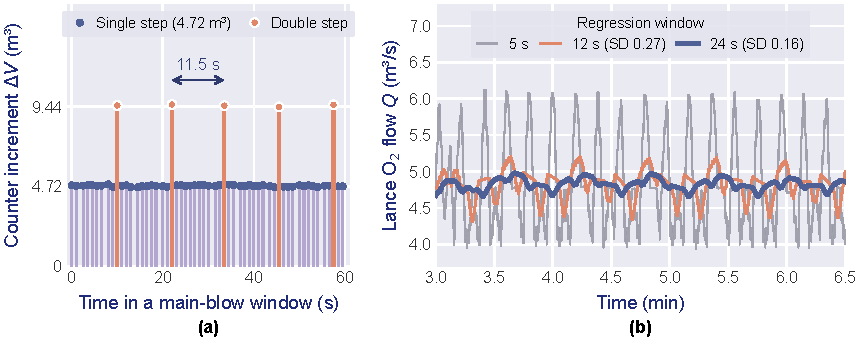
\includegraphics[width=1.0\linewidth]{figures/fig04_o2_counter_beat.pdf}
\caption{Oxygen-counter beat artifact in Heat 3: (a) counter increments; (b) sliding-window flow slopes.}\label{fig:4}
\end{figure}

\subsection{Carbon–Oxygen Balance Check}\label{sec:3.4}

The problem describes the CO and CO\ensuremath{_{2}} values as volume flow rates in m\ensuremath{^{3}}/s. We test this reading with a carbon–oxygen balance. Producing one volume of CO consumes half a volume of O\ensuremath{_{2}}, and producing one volume of CO\ensuremath{_{2}} consumes one volume of O\ensuremath{_{2}}. Under the flow-rate interpretation, the apparent ratio of stoichiometric oxygen demand to blown oxygen supply is

\begin{equation}
\alpha_{\mathrm{app}} = \frac{0.5\,E_{\mathrm{CO}}(t_{\mathrm{end}}) + E_{\mathrm{CO_2}}(t_{\mathrm{end}})}{V(t_{\mathrm{end}})}, \label{eq:massbal}
\end{equation}

where $t_{\mathrm{end}}$ denotes the end of the blow. Figure~\ref{fig:5} shows that $\alpha_{\mathrm{app}}$ lies between 5.46 and 6.53 across all ten heats, with a mean of 5.92 and a coefficient of variation of 6.5\%.

The ratio in Equation~(\ref{eq:massbal}) cannot exceed one if the readings are flow rates. During the main blow, however, $y_{\mathrm{CO}} + y_{\mathrm{CO_2}}$ stays between 49 and 61 and remains at or below 72, which matches typical converter off-gas composition in percent by volume. We therefore interpret the readings as volume fractions. The cumulative emissions required by Task 2 are still computed as time integrals of the readings, and our later conclusions rely on relative changes rather than on absolute gas volumes. If all blown oxygen leaves the bath as CO and CO\ensuremath{_{2}}, the stable ratio across heats implies an effective diluted flue-gas flow of about 16.9 m\ensuremath{^{3}}/s. Its narrow spread also indicates that the measurement chain behaves consistently across heats, supporting a common delay model.

\begin{figure}[!htbp]
\centering
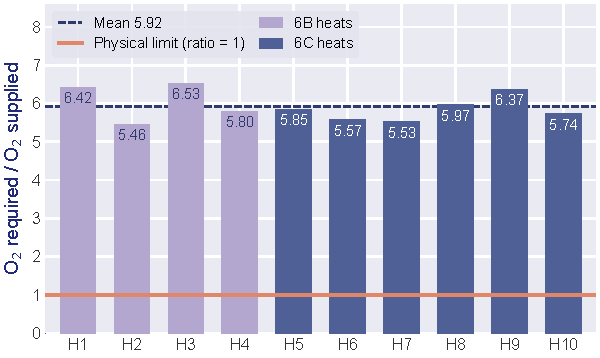
\includegraphics[width=0.7\linewidth]{figures/fig05_carbon_oxygen_balance.pdf}
\caption{Carbon–oxygen mass-balance ratio across the ten heats.}\label{fig:5}
\end{figure}


\FloatBarrier
\section{Delay-Aware Dual-Modal Framework}\label{sec:4}

All three tasks hinge on synchronizing an instantaneous optical observation at the furnace mouth with its delayed chemical signature at the gas analyzer. We formalize this coupling through a Lagrangian arrival-time map indexed by cumulative oxygen consumption $V(t)$. Under Assumption 1, each fluid element exits the exhaust hood and traverses the ductwork in sequence with minimal axial back-mixing, so it arrives at the sampling bend once the cumulative off-gas volume formed after time $t$ equals the effective duct capacity. Because Assumption 2 links off-gas production linearly to the oxygen injection rate $Q(t)$, that residence-volume balance translates directly into an oxygen-volume conservation law:

\begin{equation}
\int_{t}^{t_{\mathrm{arr}}(t)} Q(s)\,\mathrm{d}s = V\bigl(t_{\mathrm{arr}}(t)\bigr) - V(t) = \Delta V_{\mathrm{pipe}}. \label{eq:1}
\end{equation}

Here $\Delta V_{\mathrm{pipe}}$ denotes the effective duct capacity expressed in equivalent cubic metres of blown oxygen, turning $V(t)$ into an intrinsic process clock valid under arbitrary lance-flow trajectories. Across any transit interval with average flow $\bar{Q}$, advection requires $\Delta V_{\mathrm{pipe}}/\bar{Q}$ seconds, defining the pure transport arrival $t_{\mathrm{arr}}(t)$. Incorporating a first-order mixing element of time constant $T_{\mathrm{mix}}$ to account for residual axial dispersion and analyzer response shifts the mean arrival by an additional $T_{\mathrm{mix}}$ seconds, yielding the steady-flow delay relation:

\begin{equation}
\tau(Q) = T_{\mathrm{mix}} + \frac{\Delta V_{\mathrm{pipe}}}{Q}. \label{eq:2}
\end{equation}

Equation~(\ref{eq:2}) renders the flow dependence required in Task 2 directly identifiable: total lag falls monotonically as lance flow rises, with its advection component scaling inversely with $Q$. Simultaneously, Equation~(\ref{eq:1}) unifies the remaining tasks by pairing each live spectral frame at $t$ with its future ground-truth target $y\bigl(t_{\mathrm{arr}}(t)\bigr)$, identifying which earlier forecast each incoming probe measurement validates, and aligning heats with disparate blowing rates onto a common cumulative-oxygen progress axis (Figure~\ref{fig:6}).

\begin{figure}[!htbp]
\centering
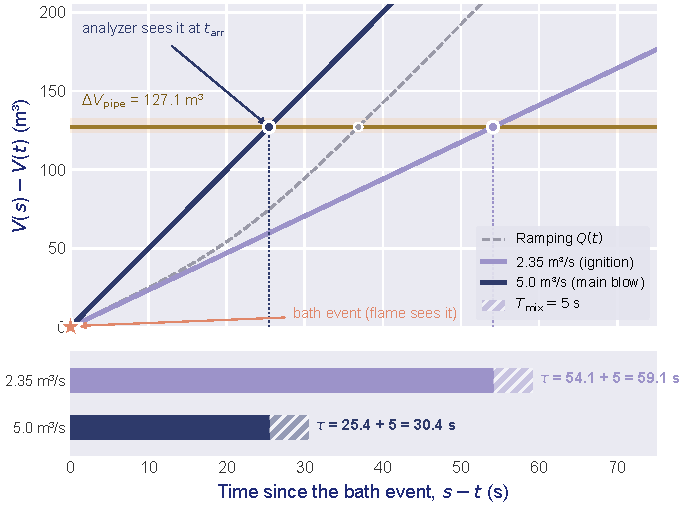
\includegraphics[width=0.8\linewidth]{figures/fig06_arrival_time_map.pdf}
\caption{Plug-flow arrival-time map under ignition and main-blow lance flows.}\label{fig:6}
\end{figure}


\FloatBarrier
\section[Task 1: Spectral Reconstruction]{Task 1: Spectral Outlier Removal and Continuous Reconstruction}\label{sec:5}

Task 1 asks for two things: the removal of outliers and a continuous surface that can be drawn in three dimensions. The data make both harder than they appear. A heat contains about 2.9 million intensity values, the flame flickers strongly from frame to frame, a few pixels saturate, and two narrow emission lines vary on their own. Filters that work along time only treat the flicker as outliers and ignore the strong correlation between neighbouring wavelengths. Ordinary principal component analysis uses this correlation but is distorted by the outliers it should detect. We therefore separate a low-rank signal from sparse outliers explicitly and build the continuous surface from the low-rank part.

\subsection{Rank-Constrained Robust Low-Rank Model (RLR)}\label{sec:5.1}

A flame spectrum is a smooth thermal continuum with a few emission lines. As the blow proceeds, the temperature and the line intensities change, but the spectral shapes stay within a small family. The log-intensity matrix of a heat is therefore nearly low-rank, while spikes and corrupted frames are sparse. RLR uses this structure in four steps.

\textbf{Step 1: Log transform and saturation mask.} We set $X_{t\lambda} = \ln I(t,\lambda)$ on the unified grid and exclude saturated pixels from the observed set; the low-rank completion of Step 4 fills them. The log transform converts multiplicative flicker into an additive shift that a single component can absorb.

\textbf{Step 2: Low-rank plus sparse decomposition.} We decompose

\begin{equation}
\mathbf{X} = \mathbf{L} + \mathbf{S} + \mathbf{N}, \qquad \operatorname{rank}(\mathbf{L}) \le r, \label{eq:3}
\end{equation}

where $\mathbf{S}$ captures sparse outliers and $\mathbf{N}$ denotes small background noise. Classical principal component pursuit \cite{ref:1} fails to separate the noise here, yielding ranks of 426–446 in every heat. We therefore fix the rank and alternate two projections \cite{ref:2}:

\begin{equation}
\mathbf{L}^{(m)} = \mathcal{P}_r\!\bigl(\mathbf{X}-\mathbf{S}^{(m-1)}\bigr), \qquad S^{(m)}_{t\lambda} = \bigl(X_{t\lambda}-L^{(m)}_{t\lambda}\bigr)\,\mathbb{1}\!\bigl(\lvert X_{t\lambda}-L^{(m)}_{t\lambda}\rvert > 5\sigma_\lambda\bigr), \label{eq:rlr_alt}
\end{equation}

where $\mathcal{P}_r(\cdot)$ denotes the rank-$r$ truncated singular value decomposition and $\sigma_\lambda$ is the wavelength-specific robust residual scale. Iteration terminates once the outlier support stabilizes.

\textbf{Step 3: Outlier rules.} We estimate $\sigma_\lambda$ separately at each wavelength via the scaled median absolute deviation, because the ultraviolet and near-infrared ends carry fewer counts and more noise. A pixel is flagged if $|X_{t\lambda}-L_{t\lambda}| > 5\sigma_\lambda$. Let $\bar{e}_t$ be the mean clipped standardized residual across wavelengths in frame $t$; the frame is flagged as anomalous when its robust z-score satisfies

\begin{equation}
Z_t = \frac{\bar{e}_t - \operatorname{med}(\bar{e})}{1.4826\,\operatorname{MAD}(\bar{e})} > 5. \label{eq:frame_z}
\end{equation}

Within an anomalous frame, we remove only the pixels with $|z|>2.5$ and keep the rest, so that the frame still determines its own low-rank scores. A run longer than 5 s is treated as a change of operation, such as the end of the blow, rather than as an outlier.

\textbf{Step 4: Continuous surface.} After removing outliers, we complete the matrix with rank $r$ and write

\begin{equation}
\hat{I}(t,\lambda) = \exp\Bigl[\mu(\lambda) + \sum_{j=1}^{r} a_j(t)\,\varphi_j(\lambda)\Bigr], \label{eq:4}
\end{equation}

where $\mu$ is the mean log spectrum, the loadings $\varphi_j$ are interpolated by cubic splines and the scores $a_j$ by smoothing splines. Equation~(\ref{eq:4}) can be evaluated at any time and wavelength, and it stays positive by construction. The smoothing parameter of $a_j$ is selected by generalized cross-validation for the reconstruction. The three-dimensional figures use a stronger smoothing ($\lambda_s = 10^4$) to display the trend of the blow.

\subsection{Model Solution and Results}\label{sec:5.2}

\subsubsection{Low-Rank Structure and Outlier Detection}\label{sec:5.2.1}

The first three components explain at least 99.6\% of the log-spectral variance in every heat, averaging 99.8\%. We select the rank by hiding 10\% of the valid pixels on two representative heats. The hold-out error drops from 0.099 at $r=1$ to 0.032 at $r=3$ and rises for larger ranks as additional components fit pixel noise. We therefore set $r=3$ for single-heat denoising. RLR flags 0.65–3.6\% of the pixels and 33–117 isolated frames per heat.

The components have a clear physical meaning. In every heat, the score of the first component follows the logarithm of the total intensity with $|r| = 1.00$, so this component measures the overall brightness of the flame. By contrast, the second score is almost independent of brightness ($|r| = 0.03$). Instead, it correlates with the intensity ratio between 800 and 500 nm ($|r| = 0.52$ on average) and with the contrast of the potassium line ($|r| = 0.48$). This component therefore describes the colour of the flame and the strength of its emission lines, two quantities related to the flame temperature.

Figure~\ref{fig:7} shows the decomposition for Heat 3. The low-rank part keeps the rise of the flame during ignition, the plateau of the main blow and the decay near the end. The sparse part concentrates on two narrow bands at 767 nm and 589 nm, the two strongest emission peaks of the mean spectrum. These lines fluctuate independently of the continuum and may correspond to the potassium doublet (766.5/769.9 nm) and the sodium D lines.

\begin{figure}[!htbp]
\centering
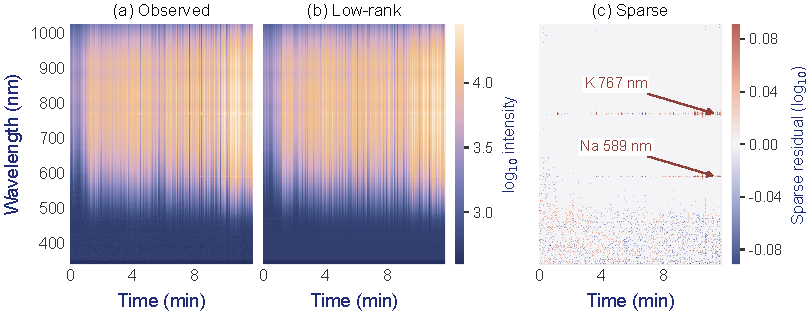
\includegraphics[width=1.0\linewidth]{figures/fig07_rlr_decomposition.pdf}
\caption{RLR decomposition of Heat 3: (a) raw log spectrum; (b) low-rank component; (c) sparse residual.}\label{fig:7}
\end{figure}

We test the detector by injecting known outliers into clean spectra of Heats 3 and 8. Spikes of 5–10 robust standard deviations hit 1\% of the pixels, and Gaussian bumps of 0.2–0.5 in log intensity distort 1\% of the frames. Table~\ref{tab:3} compares RLR with a one-dimensional Hampel filter \cite{ref:3}; higher F1 and lower error are better. RLR finds 93\% of the spikes with a precision of 87\%, while the Hampel filter mistakes flicker for spikes and misses most of them. The Hampel filter also cannot recognize distorted frames, because it judges each frame by its total intensity. Removing the detected outliers lowers the reconstruction error on the corrupted pixels from 0.068 to 0.041.

\begin{table}[!htbp]
\centering\small
\caption{Detection of injected outliers (mean of three repetitions on Heats 3 and 8)}\label{tab:3}
\renewcommand{\arraystretch}{1.12}
\begin{tabularx}{\linewidth}{@{}Z K{.13\linewidth} K{.13\linewidth} K{.10\linewidth} K{.10\linewidth} K{.18\linewidth}@{}}
\toprule
\textbf{Detector} & \textbf{Spike precision} & \textbf{Spike recall} & \textbf{Spike F1} & \textbf{Frame F1} & \textbf{Error on corrupted pixels} \\
\midrule
Hampel filter & 0.255 & 0.190 & 0.218 & 0.000 & 0.073 \\
RLR (ours) & 0.868 & 0.928 & \textbf{0.891} & \textbf{0.769} & \textbf{0.041} \\
No outlier removal & – & – & – & – & 0.068 \\
\bottomrule
\end{tabularx}
\end{table}

\subsubsection{Reconstruction Accuracy}\label{sec:5.2.2}

We evaluate reconstruction by hiding 10\% of the valid pixels and predicting them from the rest; Table~\ref{tab:4} lists the errors, where lower is better. RLR reaches a log error of 0.031, which corresponds to a relative intensity error of 2.0\%. Methods that work along time only, such as linear interpolation and Savitzky–Golay filtering, give errors above 0.36. The two-dimensional Whittaker smoother \cite{ref:4} gives 0.157. Using the spectral correlation across wavelengths is therefore the key to accurate completion.

\begin{table}[!htbp]
\centering\small
\caption{Hold-out reconstruction error (10\% of valid pixels, mean of ten heats and three repetitions)}\label{tab:4}
\renewcommand{\arraystretch}{1.12}
\begin{tabularx}{\linewidth}{@{}Z c c@{}}
\toprule
\textbf{Method} & \textbf{RMSE (log intensity)} & \textbf{Relative error} \\
\midrule
Linear interpolation in time & 0.360 & 26.6\% \\
Savitzky–Golay filter in time & 0.401 & 30.8\% \\
2-D Whittaker smoother & 0.157 & 10.6\% \\
Low-rank completion without outlier removal & 0.033 & 2.2\% \\
\textbf{RLR (ours)} & \textbf{0.031} & \textbf{2.0\%} \\
\bottomrule
\end{tabularx}
\end{table}

When whole frames are hidden, every method reaches an error of about 0.36 (RLR: 0.362; linear interpolation: 0.364). This floor reflects the frame-to-frame flicker of the flame, whose standard deviation around the trend surface is 0.30–0.71 in log intensity. The flicker comes from turbulent combustion at the mouth and cannot be inferred from neighbouring frames, so Equation~(\ref{eq:4}) represents it as the residual around a continuous trend. Figure~\ref{fig:8} shows a detected anomalous frame and the reconstruction at 600 nm.

\begin{figure}[!htbp]
\centering
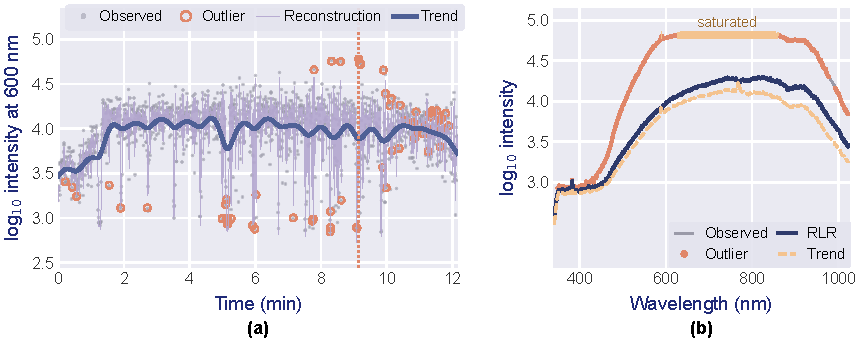
\includegraphics[width=1.0\linewidth]{figures/fig08_outlier_reconstruction.pdf}
\caption{Outlier detection and reconstruction in Heat 9: (a) 600 nm series; (b) anomalous bright frame at 9.14 min.}\label{fig:8}
\end{figure}

\subsubsection{Continuous 3D Spectral Surfaces}\label{sec:5.2.3}

Figure~\ref{fig:9} presents the continuous spectral surfaces of the ten heats. All heats share the same pattern. A dark ignition stage of 1–2 min ends with a sharp rise as the main blow starts. A broad plateau with its maximum between 750 and 900 nm follows, and the intensity declines at the end of the blow. The 6C heats reach higher intensities than the 6B heats and show more saturation, which agrees with the different instrument settings identified in Section~\ref{sec:3.1}. The timing of the rise and the decline matches the stage breakpoints found from the gas data in Section~\ref{sec:6.2}, which shows that the flame and the gas describe the same process.

\ifpaperappendix Appendix~\ref{app:heat-figures} contains the individual spectral surfaces.\fi
\begin{figure}[!htbp]
\centering
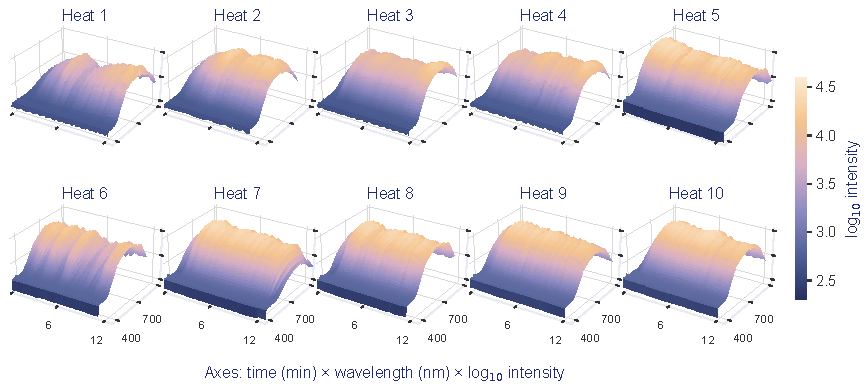
\includegraphics[width=1.0\linewidth]{figures/fig09_spectral_surfaces.pdf}
\caption{Continuous 3D spectral trend surfaces of the ten heats ($\log_{10}$ intensity).}\label{fig:9}
\end{figure}



\FloatBarrier
\section[Task 2: Process Signals and Variable Delay]{Task 2: Oxygen–Gas Relationship and Variable Flue-Gas Delay}\label{sec:6}

Task 2 contains three questions of increasing depth: how to recover continuous process curves, how the gas depends on the oxygen consumption, and how the delay depends on the lance flow. The first two describe the gas as a function of the blow; the third needs a model of the duct. We answer them in this order, because the stage structure found in the second step also locates the events used to check the delay.

\subsection{Continuous Reconstruction of the Process Signals}\label{sec:6.1}

The lance flow $Q(t)$ comes from the 24-s regression slope of Section~\ref{sec:3.3}, and $V(t)$ is the monotone cubic interpolation of the counter updates. For the gas readings, we remove two kinds of outliers. Stuck readings are runs that stay constant for more than 10 s during the active blow; we find five such runs of 22–94 points. Spikes are detected by a Hampel filter applied to the sequence of value updates, with a floor equal to the measurement noise, which flags at most four points per heat. The cleaned readings are reconstructed by monotone cubic interpolation followed by a smoothing spline. Hiding 10\% of the updates gives a reconstruction error of 0.20 for CO (mean 31.0) and 0.10 for CO\ensuremath{_{2}} (mean 13.8), both below 1\%. From the continuous curves, the lance flow and cumulative gas emissions follow directly as

\begin{equation}
Q(t) = \frac{\mathrm{d}V(t)}{\mathrm{d}t}, \qquad E_g(t) = \int_{0}^{t} y_g(s)\,\mathrm{d}s, \qquad g \in \{\mathrm{CO},\,\mathrm{CO_2}\}, \label{eq:cum_emiss}
\end{equation}

evaluated numerically via the 24-s sliding slope for $Q(t)$ and trapezoidal integration for $E_g(t)$.

Figure~\ref{fig:10} shows the six curves of Heat 3. The flow holds at about 2.4 m\ensuremath{^{3}}/s during ignition, steps up to about 4.8 m\ensuremath{^{3}}/s in the main blow and rises again near the end. CO\ensuremath{_{2}} peaks within the first three minutes, whereas CO rises later and stays high until the end of the blow. The cumulative emissions therefore grow in opposite orders: the CO\ensuremath{_{2}} curve rises early and flattens, and the CO curve starts slowly and steepens.

\ifpaperappendix The remaining nine process plots are in Appendix~\ref{app:heat-figures}.\fi
\begin{figure}[!htbp]
\centering
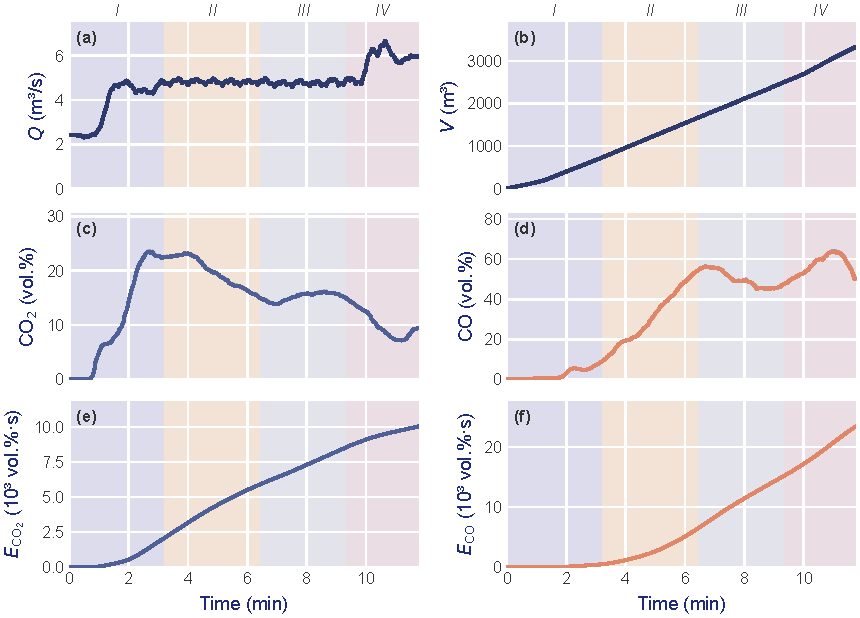
\includegraphics[width=1.0\linewidth]{figures/fig10_process_curves_heat03.pdf}
\caption{Continuous process curves of Heat 3: (a) lance flow; (b) cumulative oxygen; (c, d) gas readings; (e, f) cumulative emissions.}\label{fig:10}
\end{figure}

\subsection{Four-Stage Relationship between Oxygen and Off-Gas}\label{sec:6.2}

We describe the gas readings as functions of the cumulative oxygen $V$ rather than of time, because $V$ measures how far the blow has progressed. The rank correlations show why a single global trend is insufficient. Averaged over the ten heats, CO correlates with $V$ at $\rho = 0.74$, whereas CO\ensuremath{_{2}} correlates at $\rho = -0.13$. After a cubic time trend is removed, the CO correlation drops to 0.38, so much of the relation is a stage effect rather than a smooth proportionality. The cumulative emissions correlate with $V$ at $\rho \approx 1.00$, but only because all three quantities increase with time.

For each heat, we therefore model $y_{\mathrm{CO}}(V)$ with a continuous three-breakpoint piecewise-linear function:

\begin{equation}
y_{\mathrm{CO}}(V) = \beta_0 + \beta_1 V + \sum_{m=1}^{3} \delta_m\,(V - V_m)_{+}, \label{eq:piecewise}
\end{equation}

where $(x)_+ = \max(x,0)$, $\delta_m$ gives the slope change at breakpoint $V_m$, and a grid search places $V_2$ before 60\% and $V_3$ after 75\% of total oxygen. The fits reach $R^2 = 0.956$–$0.997$. Table~\ref{tab:5} lists the results.

\begin{table}[!htbp]
\centering\small
\caption{Four blowing stages identified from CO versus cumulative oxygen (ten heats)}\label{tab:5}
\renewcommand{\arraystretch}{1.12}
\begin{tabularx}{\linewidth}{@{}Z K{.24\linewidth} K{.22\linewidth} Z@{}}
\toprule
\textbf{Stage} & \textbf{Range of $V/V_{\mathrm{end}}$} & \textbf{CO share in CO+CO\ensuremath{_{2}}} & \textbf{Mean slope of $y_{\mathrm{CO}}$ (per m\ensuremath{^{3}})} \\
\midrule
I. Early blow (CO\ensuremath{_{2}}-dominated) & 0–0.23 (\ensuremath{\pm}0.02) & 9.5–28.9\% & 0.012 \\
II. Decarburization ramp-up & 0.23–0.43 (\ensuremath{\pm}0.06) & 51.0–61.3\% & 0.055 \\
III. Steady decarburization & 0.43–0.90 (\ensuremath{\pm}0.08) & 72.7–80.6\% & \ensuremath{-}0.002 \\
IV. End-of-blow decline & 0.90–1.00 & 57.8–84.7\% & \ensuremath{-}0.082 \\
\bottomrule
\end{tabularx}
\end{table}

The four stages follow converter bath chemistry. During Stage I, silicon and manganese consume much of the blown oxygen, and carbon oxidized at low bath temperature leaves primarily as CO\ensuremath{_{2}}. As the bath heats up in Stage II, decarburization accelerates and CO rises by 0.055 percentage points per cubic metre of oxygen. Stage III forms a steady plateau where CO remains nearly flat and accounts for roughly three quarters of the carbon-bearing off-gas. Finally, carbon depletion in Stage IV causes CO to decline sharply. The cumulative emissions follow the same breakpoints: a piecewise-linear fit of $E_{\mathrm{CO}}(V)$ and $E_{\mathrm{CO_2}}(V)$ reaches $R^2 = 0.998$ with a lower AIC than logistic or quadratic fits. Between the two converter groups, only the Stage III slope differs significantly (Mann–Whitney test, $p = 0.02$).

Figure~\ref{fig:11} shows the piecewise fits for the ten heats.
\begin{figure}[!htbp]
\centering
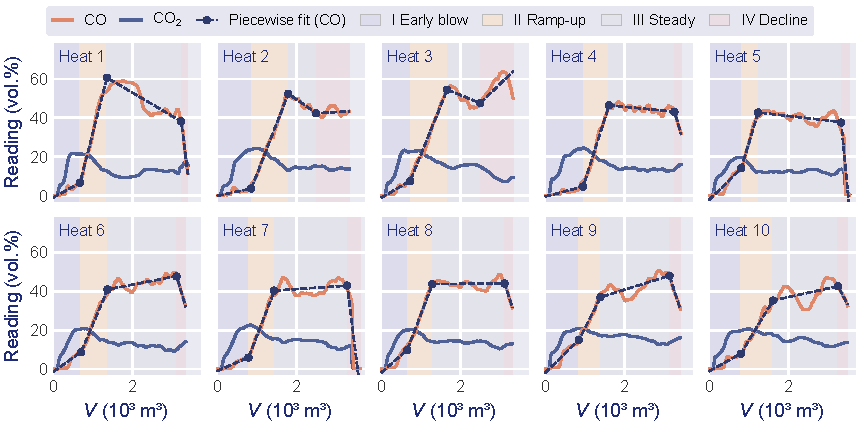
\includegraphics[width=1.0\linewidth]{figures/fig11_four_stage_relation.pdf}
\caption{Four-stage piecewise-linear CO and CO\ensuremath{_{2}} trajectories against cumulative oxygen.}\label{fig:11}
\end{figure}

\subsection{Plug-Flow Delay Model (PFD)}\label{sec:6.3}

To estimate $\Delta V_{\mathrm{pipe}}$ in Equation~(\ref{eq:1}), we need a signal whose shape is common to all heats, so that the shift between heats and their own oxygen clock can be identified. We use the oxygen-equivalent gas signal $y_{\mathrm{ox}} = y_{\mathrm{CO_2}} + 0.5\,y_{\mathrm{CO}}$, which measures the oxygen bound in the carbon gas. By the balance of Section~\ref{sec:3.4}, its time integral is proportional to the oxygen supplied, with a ratio that varies by only 6.5\% between heats. In the oxygen coordinate, the ten heats indeed share one trajectory (Figure~\ref{fig:12}b). PFD describes this trajectory in three steps.

\textbf{Step 1: Shifted generation curve.} The gas reaching the analyzer at cumulative oxygen $V$ was generated at $V^{+} = \max(V-\Delta V_{\mathrm{pipe}},\,0)$. We write the generation curve as

\begin{equation}
u(V) = g(V)\,\bigl[\eta + (1-\eta)\,s\bigl((V^{+}-V_{\mathrm{m}})/w_{\mathrm{m}}\bigr)\bigr]\; s\bigl(-(V^{+}-V_{\mathrm{e}})/w_{\mathrm{e}}\bigr), \label{eq:5}
\end{equation}

where $s(\cdot)$ is the logistic function and $g(V) = s\bigl((V-\Delta V_{\mathrm{pipe}})/3.5\bigr)$ switches the signal on when the first gas arrives. The parameter $\eta$ sets the ignition level, $(V_{\mathrm{m}}, w_{\mathrm{m}})$ locates the main-blow rise, and $V_{\mathrm{e}}$ locates the end-of-blow decline with a transition width $w_{\mathrm{e}}$ fixed at 180 m\ensuremath{^{3}}.

\textbf{Step 2: Mixing and scaling.} A first-order mixing stage with time constant $T_{\mathrm{mix}}$ maps the shifted curve $u$ to the modelled oxygen-equivalent response $\tilde{y}_{\mathrm{ox}}$ via

\begin{equation}
y_{\mathrm{ox}}(t) = y_{\mathrm{CO_2}}(t) + 0.5\,y_{\mathrm{CO}}(t), \qquad T_{\mathrm{mix}}\,\frac{\mathrm{d}\tilde{y}_{\mathrm{ox}}}{\mathrm{d}t} + \tilde{y}_{\mathrm{ox}}(t) = c_k\,u\bigl(V(t)\bigr), \label{eq:pfd_mix}
\end{equation}

where $c_k$ is a heat-specific scale factor fitted linearly against the observed $y_{\mathrm{ox}}(t)$.

\textbf{Step 3: Estimation.} We minimize the mean of $1-R^2$ over the heats with L-BFGS-B \cite{ref:5} from three starting points far from each other. Because the five parameters differ by four orders of magnitude, we rescale them to unit size before optimization. We fix the mixing constant $T_{\mathrm{mix}}$ at 5 s, because fits with 2, 5 and 10 s reach the same $R^2$ (0.9754–0.9760). The uncertainty of $\Delta V_{\mathrm{pipe}}$ comes from 250 bootstrap resamples of whole heats \cite{ref:6}, each refitting all five parameters. A synthetic test checks the estimator: data generated with $\Delta V_{\mathrm{pipe}} = 135$ m\ensuremath{^{3}} and noise are fitted from blind starting points of 45 and 210 m\ensuremath{^{3}}, and the estimate returns 135.3 m\ensuremath{^{3}}.

\subsection{Model Solution and Results}\label{sec:6.4}

\subsubsection{Duct Volume and the Delay Curve}\label{sec:6.4.1}

PFD gives $\Delta V_{\mathrm{pipe}} = 127.1$ m\ensuremath{^{3}} with a 95\% bootstrap interval of 123.4–132.6 m\ensuremath{^{3}} and a global $R^2$ of 0.976. The estimate is stable: calibrating it ten times, each time without one heat, gives 127.1 \ensuremath{\pm} 0.9 m\ensuremath{^{3}}. Substituting it into Equation~(\ref{eq:2}) gives

\begin{equation}
\tau(Q) = 5 + \frac{127.1}{Q}\ \text{s}. \label{eq:6}
\end{equation}

Table~\ref{tab:6} evaluates Equation~(\ref{eq:6}) at typical flows. At the ignition flow of 2.35 m\ensuremath{^{3}}/s, the gas needs 59 s to reach the analyzer; in the main blow at 5 m\ensuremath{^{3}}/s, it needs 30 s. Doubling the flow from 3 to 6 m\ensuremath{^{3}}/s shortens the delay by 21 s. Fitting the 6B and 6C groups separately changes the transport time by at most 0.2 s.

\begin{table}[!htbp]
\centering\small
\caption{Flue-gas delay at different lance flow rates (PFD, 95\% bootstrap interval)}\label{tab:6}
\renewcommand{\arraystretch}{1.12}
\begin{tabularx}{\linewidth}{@{}Z Z Z@{}}
\toprule
\textbf{$Q$ (m\ensuremath{^{3}}/s)} & \textbf{$\tau$ (s)} & \textbf{95\% interval (s)} \\
\midrule
2.35 & 59.1 & 57.5–61.4 \\
3.0 & 47.4 & 46.1–49.2 \\
4.0 & 36.8 & 35.8–38.2 \\
4.75 & 31.8 & 31.0–32.9 \\
5.0 & 30.4 & 29.7–31.5 \\
5.5 & 28.1 & 27.4–29.1 \\
6.0 & 26.2 & 25.6–27.1 \\
7.0 & 23.2 & 22.6–23.9 \\
\bottomrule
\end{tabularx}
\end{table}

\begin{figure}[!htbp]
\centering
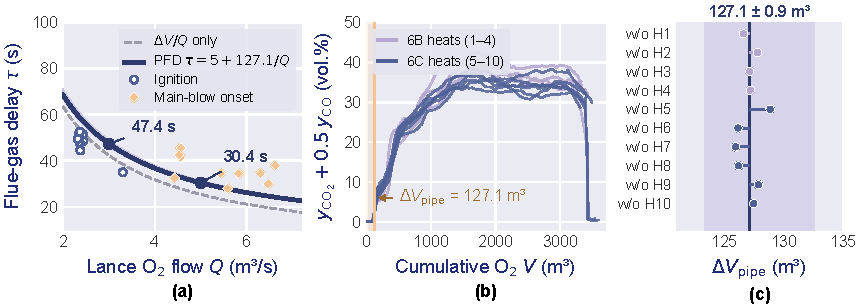
\includegraphics[width=1.0\linewidth]{figures/fig12_plug_flow_delay.pdf}
\caption{Plug-flow delay model: (a) delay curve $\tau(Q)$; (b) oxygen-equivalent trajectory collapse; (c) leave-one-heat-out $\Delta V_{\mathrm{pipe}}$.}\label{fig:12}
\end{figure}

\subsubsection{Validation against Main-Blow Onset Events}\label{sec:6.4.2}

The value of $\Delta V_{\mathrm{pipe}}$ is anchored mainly by the arrival of the first gas after ignition. Because ignition itself takes some time, we check the model against the main blow (Table~\ref{tab:7}). When the lance flow first exceeds 3.5 m\ensuremath{^{3}}/s, the oxygen-equivalent signal crosses 13 vol.\% after 28–45.5 s in the ten heats, with a median of 34.5 s. These event times include the build-up of decarburization, so they bound the transport delay from above. For the mean flows of 4.4–6.6 m\ensuremath{^{3}}/s over these intervals, Equation~(\ref{eq:6}) gives 24–34 s, below the bound as expected. A regression of all twenty ignition and main-blow events on $1/Q$ reaches $R^2 = 0.74$.

\subsubsection{Model-Free Check by Windowed Cross-Correlation}\label{sec:6.4.3}

This check requires no transport model. A cross-correlation between the first spectral component and CO over 120-s windows yields 44 windows with a distinct peak. Their delay decreases as window-mean flow increases (Spearman $\rho = -0.75$, $p = 3.4\times10^{-9}$), falling from 89 s below 4.5 m\ensuremath{^{3}}/s (three windows) and 63 s at 4.5–5.0 m\ensuremath{^{3}}/s to 31 s at 5.0–5.5 m\ensuremath{^{3}}/s and 14.5 s above 5.5 m\ensuremath{^{3}}/s (Figure~\ref{fig:13}). Because window time correlates only weakly with flow ($\rho = -0.12$), this decline is not a stage artifact.

\begin{table}[!htbp]
\centering\small
\caption{Delay estimates from independent methods}\label{tab:7}
\renewcommand{\arraystretch}{1.12}
\begin{tabularx}{\linewidth}{@{}Z K{.26\linewidth} Z@{}}
\toprule
\textbf{Method} & \textbf{Flow range (m\ensuremath{^{3}}/s)} & \textbf{Delay (s)} \\
\midrule
PFD, Equation~(\ref{eq:6}) & 5.0 & 30.4 (29.7–31.5) \\
Main-blow onset events (10 events, upper bound) & 4.4–6.6 & 28–45.5, median 34.5 \\
Windowed cross-correlation (44 windows) & 3.2–5.7 & median 40.5; decreases with $Q$, $\rho=-0.75$ \\
Constant delay maximizing spectral predictability & full blow & 31 \\
First gas after ignition (upper bound) & 2.35 & median 49.8 \\
\bottomrule
\end{tabularx}
\end{table}

\begin{figure}[!htbp]
\centering
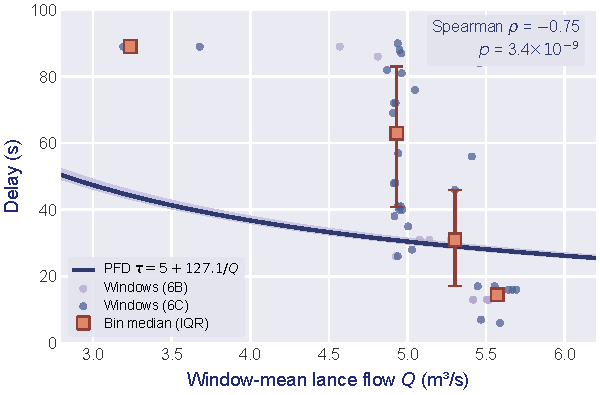
\includegraphics[width=0.7\linewidth]{figures/fig13_windowed_delay_vs_flow.pdf}
\caption{Windowed cross-correlation delay estimates versus lance flow with PFD fit.}\label{fig:13}
\end{figure}

The windowed estimates fall faster with the flow than $1/Q$ does. This suggests that the duct volume is not the only factor; a higher flow may also enhance mixing and post-combustion in the hood. In the main-blow flow range of 4.4–6.6 m\ensuremath{^{3}}/s, Equation~(\ref{eq:6}) gives 24–34 s. These values stay below the two event-based upper bounds and agree with the constant delay of 31 s that maximizes spectral predictability. We therefore adopt Equation~(\ref{eq:6}) as the delay model for Task 3 and test the consequence of a \ensuremath{\pm}10\% error in $\Delta V_{\mathrm{pipe}}$ in Section~\ref{sec:8}.



\section[Task 3: Real-Time Off-Gas Prediction]{Task 3: Real-Time Off-Gas Prediction from Flame Spectra}\label{sec:7}

Task 3 combines the low-rank spectral structure of Section~\ref{sec:5} with the delay model of Section~\ref{sec:6}. It differs from an ordinary regression in four ways. The target is delayed, so the flame at time $t$ must be matched with the gas that the analyzer reports $\tau$ seconds later. Only ten heats are available, and a model learned on one heat fails on another. The problem requires the heat-wise models to be combined. Finally, a real-time model may use only past data, and its evaluation must not let the test heat leak into any tuning step. Our soft sensor addresses these four points in turn.

\subsection{Prediction Target and Causal Features}\label{sec:7.1}

At time $t$, the flame reflects the bath state at $t$, whereas the analyzer reports that gas only after plug-flow transit at $t_{\mathrm{arr}}(t)$. We therefore define the real-time target as the delay-aligned reading $y\bigl(t_{\mathrm{arr}}(t)\bigr)$ from Equation~(\ref{eq:1}), providing a prediction roughly 25–30 s before the analyzer measurement arrives.

All features use measurements up to time $t$ only. For each frame, we subtract the ultraviolet dark baseline below 385 nm, smooth along wavelength and resample onto 127 points between 380 and 1010 nm to trim noisy spectral edges. RLR serves the offline analysis of Task 1, where saturated pixels are simply filled. An online predictor should also respect that a saturated pixel lies above the detector limit. We therefore clean the training spectra with a censoring-aware variant of the same low-rank idea. It applies a soft-thresholded rank-12 SVD to the log spectra, keeps every filled saturated pixel at or above the saturation level and then smooths along wavelength\ifpaperappendix\ (Appendix~\ref{app:code})\fi. We pool the cleaned spectra of all training heats and both converters and extract an eight-dimensional basis. It is wider than the three components of a single heat because it must also cover the differences between heats and converters. Projecting each new frame onto this basis (excluding saturated pixels) compresses 127 correlated channels into eight scores.

Three physical descriptors complement the scores: spectral centroid, spectral entropy, and a Wien colour temperature $T_{\mathrm{c}}(t)$ estimated across three line-free continuum windows (480–575, 610–750 and 785–960 nm) with $c_2 = 14{,}388$ µm·K. To suppress rapid flicker while preserving multi-scale trends causally, each descriptor $f(t)$ is smoothed by exponential moving averages at timescales of 5, 25, 80 and 200 s:

\begin{equation}
\ln\!\bigl(I(t,\lambda)\lambda^{5}\bigr) = a_0(t) - \frac{c_2}{T_{\mathrm{c}}(t)}\,\frac{1}{\lambda}, \qquad \bar{f}_{\gamma}(t) = \gamma\,f(t) + (1-\gamma)\,\bar{f}_{\gamma}(t-\Delta t), \label{eq:wien_ema}
\end{equation}

where $\gamma = 1 - \exp(-\Delta t / \tau_{\mathrm{ema}})$ sets each causal decay rate, and causal process features further supply $V(t)$, lance flow and blowing progress.

\subsection{Dual-Modal Soft Sensor (DSS)}\label{sec:7.2}

\textbf{Step 1: Linear-tree predictor.} Pure tree ensembles cannot extrapolate beyond the training range, which matters for Heat 1 because its CO reading is the highest of all heats between 30\% and 65\% of total oxygen and peaks at 59 near mid-blow. We therefore combine a ridge linear head on bounded features with gradient-boosted residual trees \cite{ref:7}:

\begin{equation}
\hat{y}(t) = \hat{\boldsymbol{\beta}}^{\top}\mathbf{x}_{\mathrm{lin}}(t) + f_{\mathrm{GBDT}}\bigl(\mathbf{x}(t)\bigr), \label{eq:hybrid}
\end{equation}

where $\hat{\boldsymbol{\beta}}^{\top}\mathbf{x}_{\mathrm{lin}}(t)$ captures global linear trends and $f_{\mathrm{GBDT}}$ fits the remaining nonlinear structure.

\textbf{Step 2: Model combination.} Models trained on a single heat fail to transfer: across all off-diagonal pairs, the median R\ensuremath{^{2}} is \ensuremath{-}0.02 and 52\% of pairs are negative. We therefore combine training heats rather than selecting one. Three schemes address the combination requirement: pooling all training heats, hard grouping by converter or cluster, and soft-gated weighting by similarity to the test heat. For the soft-gated scheme, let $\mathbf{d}_j$ be a fingerprint of heat $j$ computed from its first 60 s: the mean normalized spectrum, mean Task-1 scores, mean flow and mean log total intensity. Training heat $j$ receives sample weight

\begin{equation}
w_j = 0.55 + 0.45\,M\,\pi_j, \qquad \pi_j \propto \exp\Bigl(-0.65\,\frac{\lVert\mathbf{d}_j-\mathbf{d}_{\mathrm{test}}\rVert^2}{\operatorname{med}_i\lVert\mathbf{d}_i-\mathbf{d}_{\mathrm{test}}\rVert^2} + 0.55\,\mathbb{1}_{\text{same group}}\Bigr), \label{eq:7}
\end{equation}

where $M$ is the number of training heats and $\sum_j \pi_j = 1$. The uniform term retains information from every heat, while the similarity term emphasizes heats with comparable ignition profiles. The fingerprint uses only the first 60 s of the test heat, so the weights are fixed one minute after ignition, before the main decarburization starts, and use no later data.

\textbf{Step 3: Validation protocol.} The outer loop runs leave-one-heat-out (LOHO) validation, so each of the ten heats is predicted by a model trained strictly without it. Every data-driven quantity, including the cross-heat spectral basis and $\Delta V_{\mathrm{pipe}}$, is recalibrated inside each fold. An inner eight-versus-one loop selects the correction gain and conformal interval width, ensuring the test heat does not enter any tuning step. Two automated tests verify this isolation: corrupting future frames of a heat leaves all earlier predictions unchanged, and corrupting the test heat leaves all trained quantities unchanged.

\textbf{Step 4: Smith-type correction.} A probe reading arriving at time $t$ verifies the earlier prediction made at $t_{\mathrm{arr}}^{-1}(t)$, following the Smith predictor for dead-time systems \cite{ref:8}. The verified error updates a smoothed bias term that corrects the current prediction:

\begin{equation}
b_k = \alpha\,e_k + (1-\alpha)\,b_{k-1}, \qquad \hat{y}_{\mathrm{c}}(t) = \hat{y}(t) + g\,b_k, \label{eq:8}
\end{equation}

where $k$ indexes the latest probe arrival up to time $t$, $e_k$ is its verified error, $\alpha$ is a smoothing factor and $g$ is the inner-loop gain. Under probe interval $N_{\mathrm{p}}$, the bias updates only when a new reading arrives.

\textbf{Step 5: Prediction interval.} Split conformal prediction \cite{ref:9} scales inner-loop residuals by a local spread estimate $\hat{s}(t)$ to form a locally adaptive 90\% prediction interval:

\begin{equation}
\mathcal{C}_{0.90}(t) = \Bigl[\max\bigl(0,\,\hat{y}(t) - \hat{q}_{0.90}\,\hat{s}(t)\bigr),\;\; \hat{y}(t) + \hat{q}_{0.90}\,\hat{s}(t)\Bigr], \label{eq:conformal}
\end{equation}

where $\hat{q}_{0.90}$ is the empirical 90\% quantile of normalized inner-loop absolute residuals.

\subsection{Model Solution and Results}\label{sec:7.3}

\subsubsection{Ablation and Model Combination}\label{sec:7.3.1}

Table~\ref{tab:8} compares the variants under LOHO, where higher R\ensuremath{^{2}} and lower RMSE indicate stronger accuracy. Delay alignment is essential: without it, spectra plus process features predict delay-aligned CO\ensuremath{_{2}} at a mean R\ensuremath{^{2}} of only 0.33; aligning targets raises R\ensuremath{^{2}} to 0.66. Pooling and soft-gated weighting achieve comparable accuracy (CO: 0.881 versus 0.873), whereas hard grouping degrades accuracy because each group retains only three to five training heats. We adopt the soft-gated model as our zero-probe DSS because it closely matches pooling across all ten heats while providing an explicit heat-combination mechanism and a unified base for Smith correction.

\begin{table}[!htbp]
\centering\small
\caption{Leave-one-heat-out performance (mean R\ensuremath{^{2}} and RMSE over ten heats)}\label{tab:8}
\renewcommand{\arraystretch}{1.12}
\begin{tabularx}{\linewidth}{@{}Z K{.15\linewidth} c c c c@{}}
\toprule
\textbf{Model} & \textbf{Probe readings saved} & \textbf{CO R\ensuremath{^{2}}} & \textbf{CO RMSE} & \textbf{CO\ensuremath{_{2}} R\ensuremath{^{2}}} & \textbf{CO\ensuremath{_{2}} RMSE} \\
\midrule
Process features only & 100\% & 0.860 & 6.46 & 0.669 & 2.46 \\
Spectra + process, unaligned & 100\% & 0.801 & 7.65 & 0.327 & 3.41 \\
Spectra + process, aligned (pooled) & 100\% & 0.881 & 6.01 & 0.663 & 2.44 \\
Grouped by converter (6B/6C) & 100\% & 0.757 & 7.73 & 0.593 & 2.69 \\
\textbf{DSS, soft-gated (zero probe)} & 100\% & \textbf{0.873} & \textbf{6.18} & \textbf{0.658} & \textbf{2.45} \\
DSS + Smith, $N_{\mathrm{p}}$ = 120 s & 99.6\% & 0.908 & 5.28 & 0.695 & 2.31 \\
DSS + Smith, $N_{\mathrm{p}}$ = 60 s & 99.2\% & 0.920 & 4.93 & 0.726 & 2.19 \\
DSS + Smith, continuous & 0\% & \textbf{0.949} & \textbf{3.85} & \textbf{0.819} & \textbf{1.74} \\
Lagged analyzer reading, continuous & 0\% & 0.916 & 4.87 & 0.538 & 2.86 \\
\bottomrule
\end{tabularx}
\end{table}

The process features alone already explain much of the CO variation, because the blowing progress determines the stage. The spectra add information within each stage. Near the stage breakpoints, the DSS lowers the CO error from 8.02 to 7.55 and improves the steady stages for both gases. In the 10\% of time with the fastest flow changes, its error exceeds that of the process-only model. The flame responds to a flow change at once, whereas the gas follows with a lag.

\subsubsection{Generalization to All Ten Heats}\label{sec:7.3.2}

Figure~\ref{fig:14} presents the LOHO predictions across all ten heats. The zero-probe DSS tracks ignition, decarburization ramp-up and end-of-blow decline in every heat. Its CO R\ensuremath{^{2}} exceeds 0.85 in seven heats and spans 0.67 to 0.97 overall. CO\ensuremath{_{2}} accuracy is lower in Heats 5 (0.33), 1 (0.39) and 9 (0.50). Heat 1 has a higher CO reading than every other heat in the first half of the main blow, while Heat 5 combines coarser 1-s sampling with the highest saturation rate.

The conformal intervals perform as designed. Without probe readings, the 90\% intervals average a half-width of 10.1 for CO and cover 87.0\% of readings. Coverage drops to 62\% in the two heats with the highest CO readings (Heats 1 and 3) and reaches 76–100\% in the remaining heats. Under continuous correction, the half-width narrows to 5.7, and coverage reaches 89.8\% for CO and 89.75\% for CO\ensuremath{_{2}}, close to the nominal target level.

\begin{figure}[!htbp]
\centering
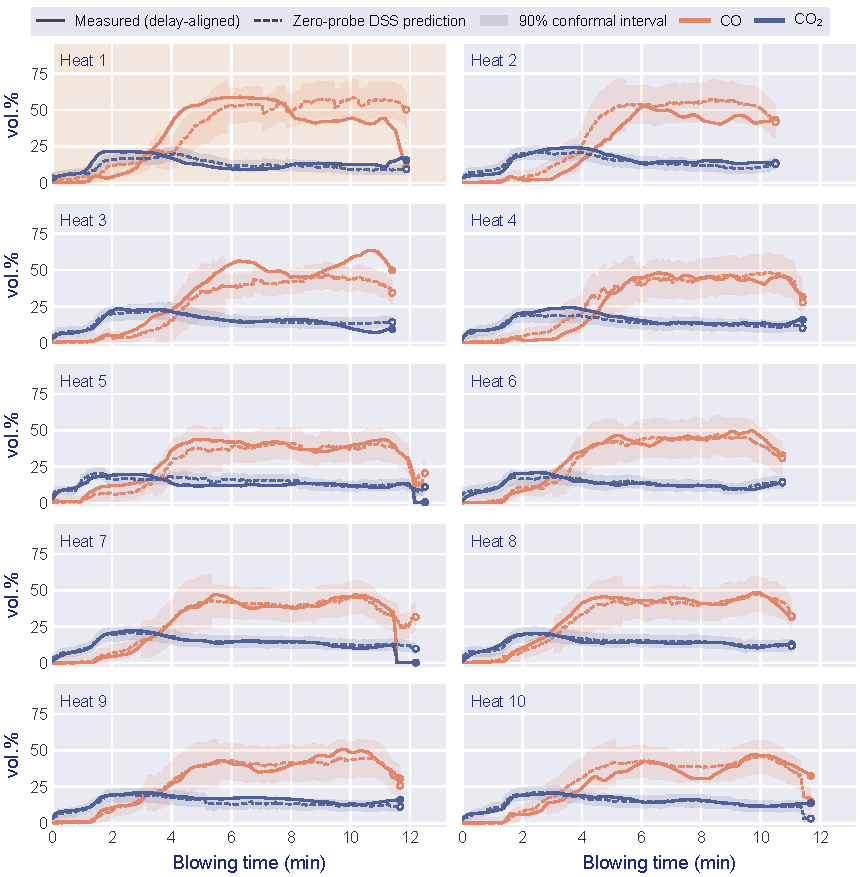
\includegraphics[width=1.0\linewidth]{figures/fig14_loho_predictions.pdf}
\caption{Leave-one-heat-out zero-probe DSS predictions with 90\% conformal intervals across all ten heats.}\label{fig:14}
\end{figure}

\subsubsection{Reducing Probe Usage}\label{sec:7.3.3}

The DSS shifts the probe from a continuous sensor to an occasional calibrator. Figure~\ref{fig:15}b plots accuracy against probe interval. With one reading every 120 s, corrected predictions reach CO R\ensuremath{^{2}} = 0.908 and CO\ensuremath{_{2}} R\ensuremath{^{2}} = 0.695, whereas holding the lagged reading yields only 0.593 and \ensuremath{-}1.04. Even under continuous sampling, the corrected prediction outperforms the lagged reading (0.949 versus 0.916 for CO) by compensating for the 30-s transport delay.

This trade-off yields clear operating points. Sampling every 60 s saves 99.2\% of probe readings while maintaining CO R\ensuremath{^{2}} at 0.920; sampling every 30 s saves 98.3\% and reaches 0.934. In a partial least squares analysis, the highest-importance wavelengths lie at 765–770 nm and 590 nm, the potassium and sodium lines isolated in Task 1, followed by the 730–825 nm continuum. The same atomic emission lines thus separate sparse outliers in Task 1 and carry off-gas information in Task 3.

\begin{figure}[!p]
\centering
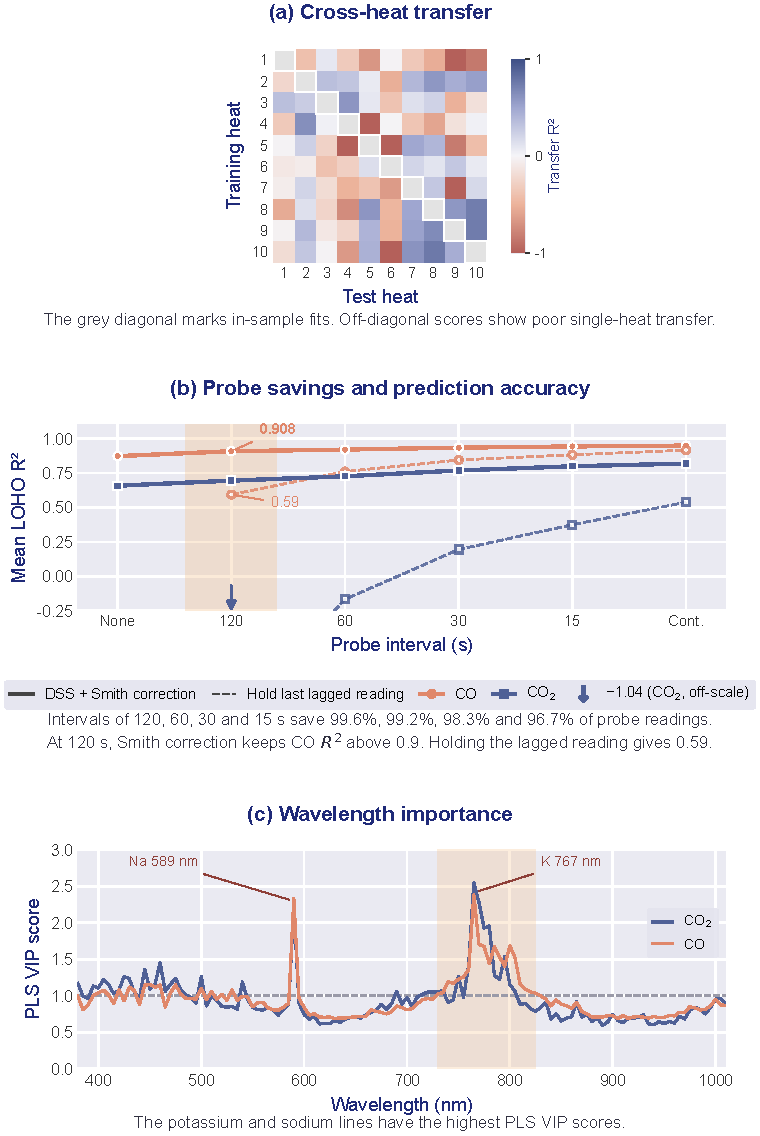
\includegraphics[width=\linewidth,height=.92\textheight,keepaspectratio]{figures/fig15_transfer_probe_vip.pdf}
\caption{Cross-heat transfer, probe-saving trade-off and wavelength importance.}\label{fig:15}
\end{figure}



\FloatBarrier
\section{Sensitivity Analysis}\label{sec:8}

We perturb the parameters that support the main conclusions and judge each perturbation by the quantity it could change. Table~\ref{tab:9} summarizes the results.

\begin{table}[!htbp]
\centering\small
\caption{Sensitivity of the main results}\label{tab:9}
\renewcommand{\arraystretch}{1.12}
\begin{tabularx}{\linewidth}{@{}K{.07\linewidth} K{.20\linewidth} K{.21\linewidth} Z@{}}
\toprule
\textbf{Task} & \textbf{Parameter} & \textbf{Values tested} & \textbf{Effect} \\
\midrule
1 & Outlier threshold & 4\ensuremath{\sigma}, 5\ensuremath{\sigma}, 6\ensuremath{\sigma} & flagged pixels 2.5\%, 2.2\%, 2.1\%; anomalous frames unchanged \\
1 & Rank $r$ & 2–6 & hold-out error 0.046, 0.032, 0.035, 0.041, 0.040 \\
2 & Mixing constant $T_{\mathrm{mix}}$ & 2, 5, 10 s & $\Delta V_{\mathrm{pipe}}$ = 131.9, 127.1, 122.0 m\ensuremath{^{3}}; $\tau$ at 4.5 m\ensuremath{^{3}}/s = 31.3, 33.3, 37.1 s \\
2 & Time step of Heat 5 & 1 s, 0.5 s & transport time changes by less than 0.5 s \\
2 & Converter group & 6B, 6C & transport time differs by at most 0.2 s \\
3 & $\Delta V_{\mathrm{pipe}}$ & \ensuremath{-}10\%, +10\% & zero-probe DSS: R\ensuremath{^{2}} changes by \ensuremath{\leq} 0.003 (CO, CO\ensuremath{_{2}}) \\
3 & $\Delta V_{\mathrm{pipe}}$ with Smith correction & \ensuremath{-}10\%, +10\% & CO R\ensuremath{^{2}} within 0.003; CO\ensuremath{_{2}} R\ensuremath{^{2}} 0.706 \ensuremath{\to} 0.755 at $N_{\mathrm{p}}$ = 60 s \\
3 & Probe interval $N_{\mathrm{p}}$ & 15–120 s, continuous & CO R\ensuremath{^{2}} 0.943–0.908, 0.949 \\
\bottomrule
\end{tabularx}
\end{table}

For Task 1, a stricter threshold removes fewer pixels but leaves the number of anomalous frames unchanged, and ranks from 3 to 6 give similar hold-out errors. The outlier rules and the rank therefore do not drive the reconstruction.

For Task 2, the mixing constant and the duct volume trade off against each other. The total delay at the main-blow flow still varies by less than 6 s, and the two converter groups share one duct model. The choice of the time step of Heat 5 also has a negligible effect.

The most critical check concerns Task 3, where the delay defines the prediction target. We perturb the duct volume by \ensuremath{\pm}10\% during both training and Smith correction while still evaluating against the calibrated target. Zero-probe accuracy shifts by at most 0.003, and corrected CO accuracy likewise stays within 0.003. By contrast, CO\ensuremath{_{2}} correction improves slightly as the assumed volume grows. This aligns with the spectral-predictability criterion, whose constant lag maximizing predictability is 72 s for CO\ensuremath{_{2}} versus 31 s for CO. Both results suggest that the CO\ensuremath{_{2}} reading follows the flame more slowly than the CO reading; the present data do not identify the cause.



\FloatBarrier
\section[Model Evaluation and Discussion]{Model Evaluation and Further Discussion}\label{sec:9}

\subsection{Strengths}\label{sec:9.1}

\begin{itemize}
\item \textbf{Data-consistency diagnosis.} Before fitting any model, we adopt the corrected Attachment 1, establish the 1-s step of Heat 5, suppress the oxygen-counter beat and show that the gas readings are volume fractions.
\item \textbf{Unified low-rank structure for cleaning and continuity.} RLR uses the same three components to detect outliers, fill saturated pixels and build continuous surfaces, with each step verified by injection testing.
\item \textbf{Physically grounded delay model.} PFD derives flow dependence from plug-flow transport. Its main-blow delay agrees with independent constant-delay estimates, stays below event-based upper bounds and matches the negative delay–flow trend from windowed cross-correlation.
\item \textbf{Strictly causal, leakage-free validation.} Every learned parameter is recalibrated within each LOHO fold, and the test heat does not enter any tuning step.
\item \textbf{Practical soft sensor.} The DSS forecasts off-gas states about 30 s ahead while keeping CO R\ensuremath{^{2}} above 0.9 with 99.6\% fewer probe readings.
\end{itemize}

\subsection{Weaknesses}\label{sec:9.2}

\begin{itemize}
\item \textbf{Limited sample of ten heats.} Heats 1 and 3 have the highest CO readings of the ten heats, so the zero-probe model extrapolates when either is held out, and coverage falls to 62\%. Additional heats, particularly high-carbon blows, would widen the training envelope.
\item \textbf{Narrow main-blow flow range.} Median lance flows across heats cluster between 4.6 and 5.1 m\ensuremath{^{3}}/s, so delay–flow identification rests on modest flow variations. Under Assumption 1, $T_{\mathrm{mix}}$ cannot be separated from $\Delta V_{\mathrm{pipe}}$ without deliberate flow steps.
\item \textbf{Undocumented gas units.} Assumption 4 relies on the carbon–oxygen balance rather than instrument manuals, leaving absolute flue-gas volume unverified until analyzer calibration records become available.
\end{itemize}

\subsection{Further Discussion}\label{sec:9.3}

Additional heats with deliberate lance-flow steps would separate $T_{\mathrm{mix}}$ from $\Delta V_{\mathrm{pipe}}$ and test the steeper power-law delay suggested by the windowed estimates. Radiometric calibration of the spectrometer would further convert colour temperature into absolute flame temperature. Moreover, pairing predicted CO with the Stage IV decline could provide an early endpoint indicator for decarburization.

Our framework transfers readily to other converters. Equation~(\ref{eq:1}) requires only cumulative oxygen and one calibrated duct volume, and the cross-heat spectral basis can be re-estimated from a handful of heats. The similarity weights in Equation~(\ref{eq:7}) then let each new heat borrow strength from comparable past blows. In plant operation, operators can select a probe interval from Figure~\ref{fig:15}b to balance probe wear against accuracy, while the conformal interval flags heats moving outside prior training experience.


\FloatBarrier
\section{Conclusions}\label{sec:10}

We developed a delay-aware framework that fuses real-time flame spectra with delayed flue-gas readings in converter steelmaking. Prior data diagnosis resolved Attachment 1, established the time step of Heat 5, eliminated the oxygen-counter beat and identified the gas readings as volume fractions.

For Task 1, our Rank-Constrained Robust Low-Rank model decomposed each log spectrum into three physical components and sparse outliers. It detected injected spikes with an F1 score of 0.89, reconstructed held-out pixels within a 2.0\% relative error and generated continuous spectral surfaces for all ten heats.

For Task 2, the reconstructed process signals revealed four blowing stages with breakpoints at 23\%, 43\% and 90\% of total oxygen. The Plug-Flow Delay model yielded $\tau(Q) = 5 + 127.1/Q$ s, which drops from 47.4 s at 3 m\ensuremath{^{3}}/s to 30.4 s at 5 m\ensuremath{^{3}}/s, and independent checks confirmed that delay decreases with flow.

For Task 3, the Dual-Modal Soft Sensor combined heat-level models through causal similarity weighting. Without probe readings, it predicted delay-aligned CO and CO\ensuremath{_{2}} at mean R\ensuremath{^{2}} of 0.873 and 0.658 across all ten heats; adding one probe reading every 120 s raised R\ensuremath{^{2}} to 0.908 and 0.695. Flame spectra can thus replace most probe readings while delivering off-gas information roughly 30 s earlier.


